\subsection{Fisher-Kernel}
\label{sec:fisher}

In 2006 Florent Perronnin and Christopher Dance proposed to use Fisher kernel for image categorization \cite{Perronnin2006}. Fisher kernels were introduced by Jaakkola and Haussler in 1999 as a method to combine the benefits of generative and discriminative approaches. They named it named after the biologist Ronald Fisher and used the fisher score from \eqnref{fisher_score} together with the kernel function \ref{eqn:fisher_kernel} (the fisher kernel) to express the similarity between multiple feature vectors. 

\begin{equation}
U_X = \nabla_\lambda \log p(X|\lambda)
\label{eqn:fisher_score}
\end{equation}
where $X = \{x_t, t = 1 \dots T\}$ is a set of low-level feature vectors and $\lambda = \{w_i, \mu_i, \Sigma_i, i = 1 \dots N\}$ a set of parameters of a \acf{GMM} ($w, \mu, \Sigma$ denote the weight, mean and covariance matrix).
\begin{equation}
K(X_i, X_j) = U_{X_i}^T I^{-1} U_{X_j}
\label{eqn:fisher_kernel}
\end{equation}
with $I = E_X\{U_X U_X^T\}$ as the Fisher information matrix (see \cite{amari1998natural} for more details). Perroninnin and Dance denoted

\begin{equation}
\mathcal{L} (X|\lambda) = \log p(X|\lambda)
\label{eqn:fisher:score2}
\end{equation}

for the usage of fisher kernels on visual vocabularies with a \ac{GMM} representation of the visual words. Where the \ac{GMM} parameters express the relative frequency $w_i$, the mean $\mu_i$ and the variation $\Sigma_i$ around the mean of the word $i$. Under an independence assumption, \eqnref{fisher:score2} corresponds to

\begin{equation}
\mathcal{L} (X|\lambda) = \sum_{t=1}^{T} \log p(x_t|\lambda)
\end{equation}

which results in the likelihood (\eqnref{fisher_likelihood}) that a observation $x_t$ was generated by the \ac{GMM}, where the weights are constrained by \ref{eqn:fisher_weights}.

\begin{equation}
p(x_t|\lambda) = \sum_{i=1}^{N} w_i p_i (x_t|\lambda)
\label{eqn:fisher_likelihood}
\end{equation}

\begin{equation}
\sum_{i=1}^{N} w_i = 1
\label{eqn:fisher_weights}
\end{equation}

The authors defined the components $p_i$ as

\begin{equation}
p_i(x|\lambda) = \frac{
	\ 	exp \{-\frac{1}{2} (x-\mu_i)' \Sigma_{i}^{-1} (x-\mu_i)\}
}{
	(2 \pi)^{D/2} | \Sigma_i |^{1/2}
}
\end{equation}

with $D$ as feature vector dimensionality and $|.|$ as determinant operator. Together with

\begin{equation}
\gamma_t(i) = p(i|x_t,\lambda) = \frac{w_i p_i(X|\lambda) }{\sum_{j=1}^{N} w_j p_j(x_t|\lambda)}
\label{eqn:fisher:gamma}
\end{equation}

which gives the probability that a feature $x_t$ was generated by the Gaussian $i$, they created the following derivations:

\begin{eqnarray}
\frac{\partial \mathcal{L} (X|\lambda)}{\partial w_i} &=& \sum_{t=1}^{T} \left[ \frac{\gamma_t(i)}{w_i} - \frac{\gamma_t(1)}{w_1} \right]
\label{eqn:fisher:derivation1}\\
\frac{\partial \mathcal{L} (X|\lambda)}{\partial \mu_i^d} &=& \sum_{t=1}^{T} \gamma_t(i) \left[ \frac{x_t^d - \mu_t^d}{(\sigma_i^d)^2} \right]
\label{eqn:fisher:derivation2}\\
\frac{\partial \mathcal{L} (X|\lambda)}{\partial \sigma_i^d} &=& \sum_{t=1}^{T} \gamma_t(i) \left[ \frac{(x_t^d - \mu_t^d)^2}{(\sigma_i^d)^3} - \frac{1}{\sigma_i^d} \right]
\label{eqn:fisher:derivation3}
\end{eqnarray}

By using the equations \ref{eqn:fisher:gamma} to \ref{eqn:fisher:derivation3}, they were able to build a \ac{BOV} which directly relates to a fisher kernel. This was possible as the \ac{BOV} representation of the relative number of occurrences of the $i$-th word can be expressed by:

\begin{equation}
\frac{1}{T} \sum \gamma_t(i)
\label{eqn:fisher:bov}
\end{equation}

The direct relation between \eqnref{fisher:derivation1} and \eqnref{fisher:bov} can be established if one consideres only the gradient with respect to the \ac{GMM} weight as both equations consider 0-th order statistics. By additionaly taking \eqnref{fisher:derivation2} and \eqnref{fisher:derivation3}, the 1-st and 2-nd order statistics will also be considered by the Fisher kernel.

As one can see in \figref{fisher_kernel_performance} Perroninnin and Dance were able get similar results for both supervised and unsupervised fisher kernels compared to a supervised \ac{BOV}. As their fisher vector approach also uses a \ac{SVM} for classification, it could be integrated seamlessly into frameworks which use other feature representations. The downside is the increased memory consumption as the resulting fisher vector size contains a multiple of the input feature dimensionality (approximately $(D*2+1)*N-1$ for $N$ \ac{GMM} components).

\begin{figure}
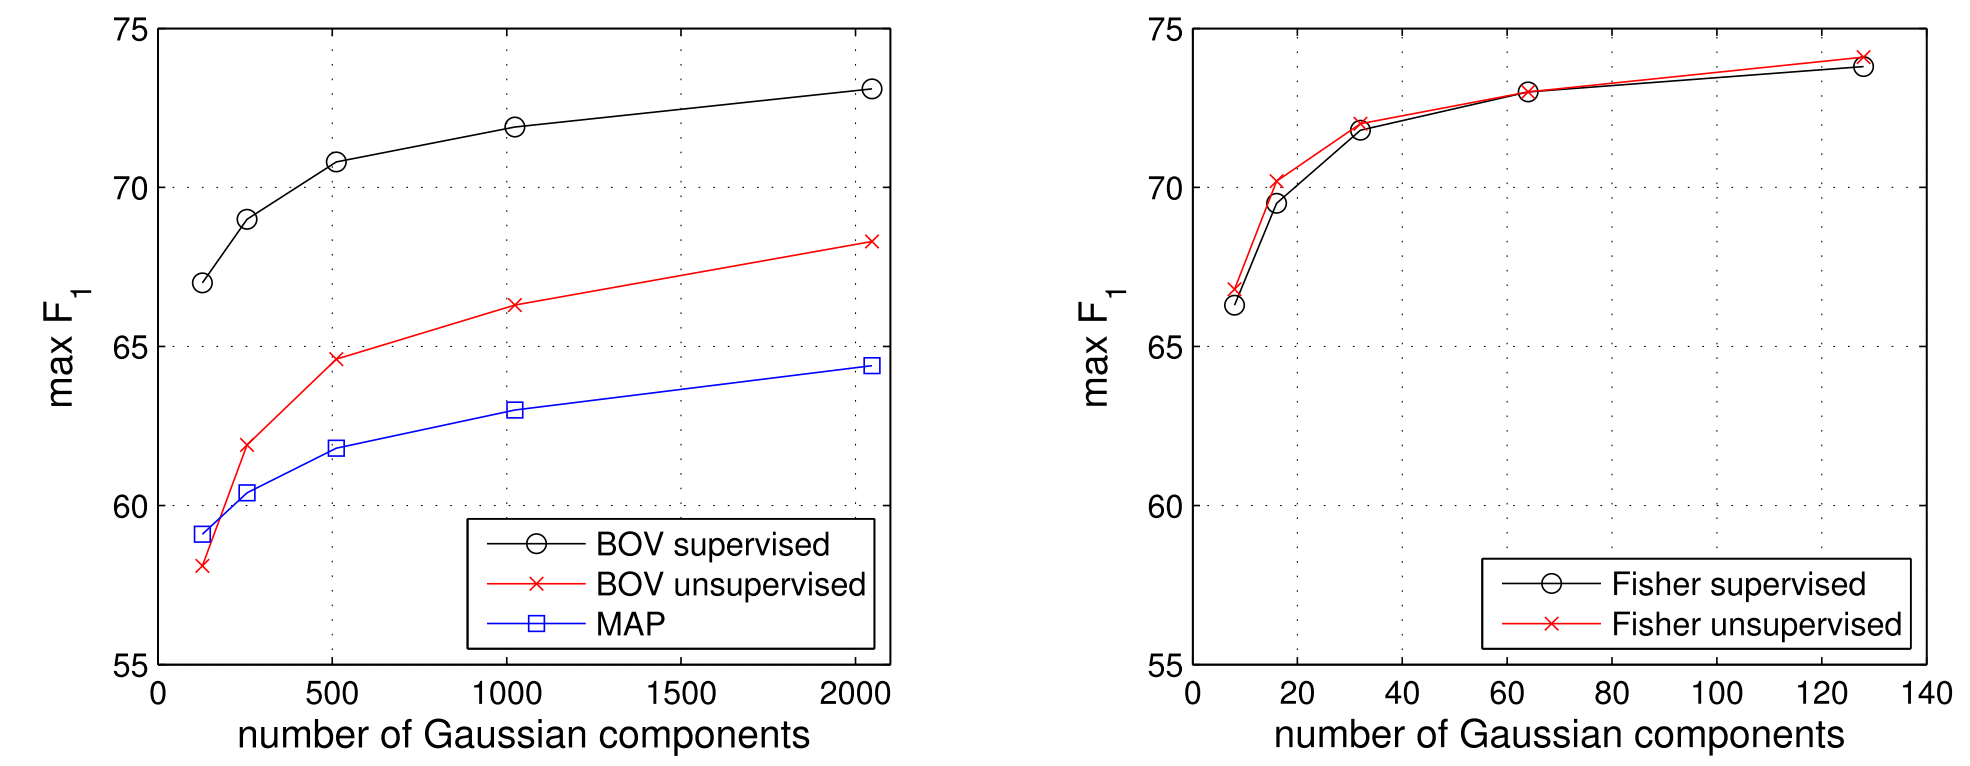
\includegraphics[width=\linewidth]{images/fisher_kernel_performance}
\caption{Performance of fisher kernels compared to a traditional \acs{BOV}.}
\label{fig:fisher_kernel_performance}
\end{figure}

\FloatBarrier